\chapter{ Impacts of past abrupt land change on local biodiversity globally}
%\addcontentsline{toc}{chapter}{Chapter 3}
%\markboth{}{Impacts of past abrupt land change on local biodiversity globally}

Abrupt land change, such as deforestation or agricultural intensification, is a key driver of biodiversity change. Following abrupt land change, local biodiversity often continues to be influenced through biotic lag effects. However, understanding of how terrestrial biodiversity is impacted by past abrupt land changes is incomplete. By combining geographically- and taxonomically-broad data on local biodiversity with quantitative estimates of abrupt land change detected within time series of satellite imagery from 1982 to 2015, here we show that abrupt land change in the past continues to influence present species assemblages globally. Species richness and abundance were reduced by 4.2\% and 2\%, respectively, and assemblage composition was altered at sites with an abrupt land change compared to unchanged sites, although impacts differed among taxonomic groups. Biodiversity recovered to levels comparable to unchanged sites after >10 years. Ignoring delayed impacts of abrupt land changes likely results in incomplete assessments of biodiversity change.

\section{Introduction}
Natural and anthropogenic processes change the terrestrial surface of the Earth \citep{Ellis2013,Song2018}, which have been shown to impact biodiversity \citep{Newbold2015,Jung2018} and ecosystem services \citep{Isbell2015}. Previous studies have found that present differences in land-surface conditions reduce local biodiversity globally \citep{Gibson2011,Newbold2015}. However, these studies often ignore the impacts of past land change \citep{Foster2003,Watson2014}. Simulations and experiments have demonstrated that land changes of greater magnitude have larger impacts on the number of species and individuals \citep{Dornelas2010,Hautier2015,Santini2016}. Yet, few studies have quantified the impacts of land change in the past on local biodiversity globally.

Local biodiversity continues to be influenced by past land change through biotic lags. Biotic lags—including ecological processes such as extinction debt \citep{Tilman1994,Kuussaari2009,Halley2016}, colonization credit \citep{Hylander2013} and ecological memory effects \citep{Ogle2015}—negatively affect the number of species and individuals present within local assemblages \citep{Halley2016,Jung2018,Perring2018}, and potentially reduce resilience \citep{Hautier2015,Nimmo2015}. The impacts of land change on species assemblages through biotic lag depend on species’ abilities to persist \citep{Turner1998} and recover \citep{Martin2013,Fu2017,Moreno-Mateos2017}. Most previous global studies \citep{Supp2014,Fu2017,Moreno-Mateos2017,Shackelford2017} investigating abrupt land changes in the past have used descriptive study-specific categories of “land changes”, e.g. wild fire, flooding or cultivation, thus hindering comparisons among studies, and preventing predictions. To assess the impacts of abrupt land change on local biodiversity more generally, comparable quantitative measures of “land change” are needed.

The availability of time series of satellite imagery enables the detection and quantification of land changes globally \citep{Kennedy2014,Song2018}. Land change can be defined as abrupt shifts in intra- and inter-annual dynamics of remotely-sensed photosynthetic activity quantified through vegetation indices \citep{Linderman2005,Pettorelli2005}. Abrupt shifts in magnitude \citep{Kennedy2012,Watson2014,DeVries2015b} and/or trend \citep{DeJong2013} of photosynthetic activity, and the time passed since such shifts \citep{POTTER2003,Kennedy2012} are three key attributes of land change \citep{Watson2014}. Several algorithms have been developed to detect abrupt land change \citep{Zhu2017} and measure these attributes. However, attributes of remotely-sensed abrupt land change have never before been used to assess biotic lags in local biodiversity.

Here we investigate the impacts of abrupt land change in the past—defined as the single largest shift in magnitude and/or trend of photosynthetic activity \citep{Verbesselt2010a,DeJong2013,Song2018}—on local biodiversity globally. We used data on local biodiversity of unprecedented geographic and taxonomic coverage from the Projecting Response of Ecological Diversity in Changing Terrestrial Systems (PREDICTS) database \citep{Hudson2016}. At each site, where local biodiversity was sampled, we assessed time series of high spatial resolution (nominal \textasciitilde30m) Landsat satellite imagery from 1982-2015 for the presence of an abrupt land change (Figure \ref{F03_01}\textbf{a}) and, where detected, we quantified key attributes, \ie, shifts in magnitude, trend and time passed. Using hierarchical analyses, we compared four measures of local biodiversity (species richness, total abundance, evenness and species turnover) between paired sites (5,563 sites with and 10,102 without an abrupt land change) from 377 studies (Figure \ref{F03_01}\textbf{b}). We expect that abrupt land changes with larger shifts in magnitude and trend have greater impacts on local biodiversity through biotic lag effects and that with more time passed local biodiversity can recover from the impacts of abrupt land change.

% ---------------- Figure 1 --------------------- %
\begin{figure}[!htb]
\centering
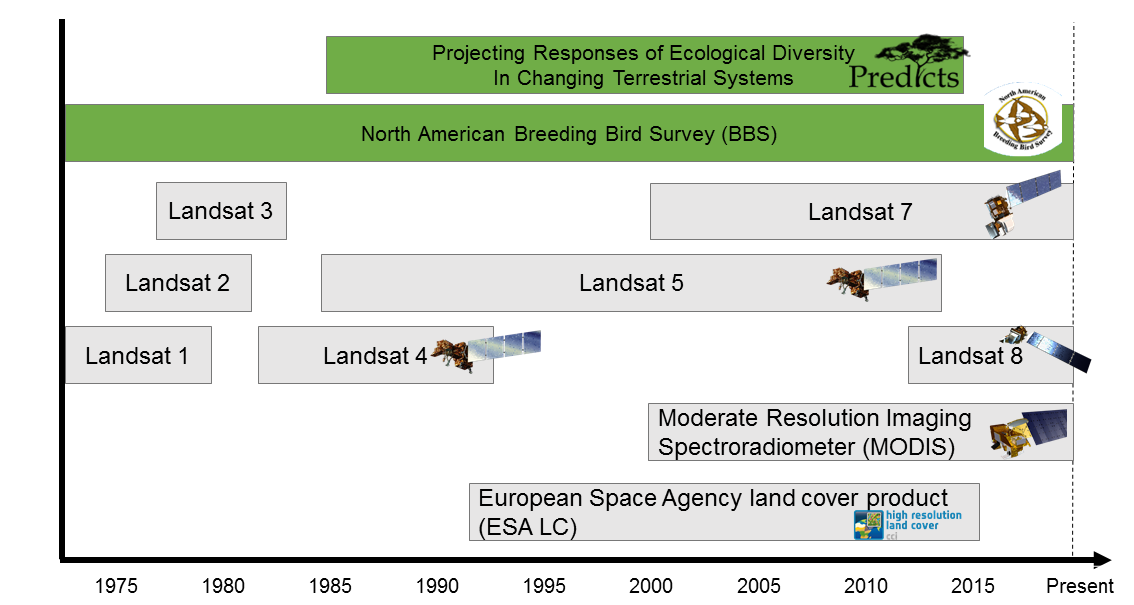
\includegraphics[width=1\textwidth]{chapter3/F01}
\caption{ Examples and distribution of sites without and with abrupt land change. (\textbf{a}) Remotely-sensed time series of monthly Enhanced Vegetation Index (EVI; green points) at an unchanged site; a site with an abrupt shift in magnitude, \ie, loss in EVI; and a site with a shift in EVI trend, \ie, an increase in annual EVI. Linear (black lines) and seasonal (dark green lines) fits of the change detection algorithm \citep{Verbesselt2010a} are shown. (\textbf{b}) Location of 5,563 sites from 377 studies in the PREDICTS database with an abrupt land change in the monitoring period (since 1982) of the Landsat 4-8 missions. Colours indicate sites with abrupt land change that had a magnitude gain (\textbf{+}) or loss (\textbf{-}) and/or trend increase (\textbf{+}) or decrease (\textbf{-}); (magnitude | trend). For ease of viewing, the location of 10,102 sites without an abrupt land change has been omitted. Latitudinal distribution of sites with an abrupt land change and time passed between abrupt land change and biodiversity sampling (in years, mean and standard deviation shown in red) by 25\textdegree  latitudinal bands. Map shown in Eckert IV equal-area projection.}
\label{F03_01}
\end{figure}
% -------------------------------------------- %
\clearpage %so that Figure 1 appears here

\section{Methods}
\subsection{Biodiversity data} 
We used data from the Projecting Responses of Ecological Diversity In Changing Terrestrial Systems (PREDICTS) database \citep{Hudson2016}, which includes species’ presence and abundance data from ‘studies’ with at least two spatially-explicit ‘sites’, information on the date of sampling, and local land-use and/or land-use intensity \citep{Hudson2016}. We simplified the original PREDICTS land use and land-use intensity information \citep{Hudson2014,Hudson2016} by allocating each site to one of three broad land-use categories: primary vegetation (\textbf{PV}, \ie primary [non-] forest), secondary vegetation (\textbf{SV}, \ie mature, intermediate, young and indeterminate age secondary vegetation) or human-dominated vegetation (\textbf{HDV}, \ie, plantation forest, cropland, pasture, urban). Studies were grouped into eight broad taxonomic groups based on the sampled taxa: plants, fungi, ground dwelling invertebrates (\eg, soil-fauna, snails, beetles), flying invertebrates (\eg, butterflies, bees, dragonflies), amphibians, reptiles, birds or mammals. 

We assessed four measures of local biodiversity that complement each other and have previously been shown to be sensitive to abrupt land change \citep{Supp2014,Santini2016}. For each site in the PREDICTS database, we calculated within-sample species richness and, where data on abundance were available, log\textunderscript{10} total abundance of individuals, adjusted by sampling effort following \cite{Newbold2014b}. After visual inspection, we removed one outlier study (a study of soil biomass, ID = \\ \detokenize{DL1_2012__CalvinoCancela}) from further analyses because of very large abundance estimates ($> 3\times10^6$ individuals). As a measure of assemblage evenness, we calculated the arcsine square root transformed probability of an interspecific encounter (PIE), which quantifies the probability of two individuals randomly chosen from an assemblage representing different species \citep{Hurlbert1971}. As a measure of turnover in species assemblage composition within studies, we calculated the S\o rensen similarity index among spatial pairs of sites within each study and land-use category \citep{Magurran2004}.

Species assemblages were sampled at various spatial extents defined by each study’s sampling method and land use. Following the PREDICTS data curation protocol we assumed the allocated land use to be dominant within the reported sampling extent (maximum linear extent [MLE], in meters) of each site \citep{Hudson2014,Hudson2016}. For studies without reported MLE (4779 sites, 18.3\% of all sites), we used either the mean MLE for each taxonomic group and corresponding sampling method, \eg, mist netting, pitfall trapping, or the mean MLE within the same taxonomic group. To test whether these interpolated MLEs are consistent among taxonomic groups and sampling method, we randomly removed 25\% of the reported MLEs and found the interpolated MLEs to be reasonably correlated (Pearson’s r = 0.73, p < 0.001). We included all studies with a MLE < 3000m (98.3\% of all sites), approximately 100 times the nominal resolution (\textasciitilde 30m) of the remotely-sensed data used in this study, and removed four studies with sites located in water (rivers, coastal areas or ponds), identified by intersecting all sites with a global permanent water surface mask \citep{Pekel2016}, as a precaution as sites within these studies likely have low positional accuracy. To spatially link species assemblage with remote sensing data, we calculated a rectangular buffer with MLE as radius (MLE\textunderscript{mean}= 412.1 m $pm$ 1,661.82m SD) around each site’s coordinates as the smallest area that fully captures all grid cells of varying sampling units (\eg, point counts, line transects). 

\subsection{Remote sensing data} 
We used land-surface reflectance products derived from the sensors of the Landsat 4 (1982 – 1993), 5 (1984 - 2012), 7 (1999 – ongoing), and 8 (2013 – ongoing) missions available within Google Earth Engine (GEE) \citep{Gorelick2017}, based on raw United States Geological Service Landsat Collection images (Tier 1) to calculate the Enhanced Vegetation Index (EVI, as two-band version \cite{Jiang2008}) as a proxy of photosynthetic activity. We masked all cloud-covered grid cells (\textasciitilde 30 m nominal resolution) using the cloud-detection output in the ‘cfMask’ band \citep{Zhu2012} and removed occasional snow- and water-covered grid cells, \ie those with negative EVI values. All data preparation and extraction were performed within GEE \citep{Gorelick2017}.

For each Landsat image and PREDICTS site we calculated the mean EVI within the rectangular buffer ($\bar{y}$) and extracted time series of all EVI values. We removed outliers introduced by satellite sensor errors, missed cloud shadows or bad quality estimates by calculating the absolute difference of all $\bar{y}$ values from the median absolute deviation (MAD) per EVI time series \citep{Leys2013}. EVI values more than a conservative threshold of two units of deviation away from the MAD or in the top 1\% of all MAD estimates were set to NA \citep{Leys2013}. Time series of EVI data were temporally aggregated to monthly maximum value composites to ensure equal intervals between data points and to reduce the amount of noise and missing data. Because of the ongoing consolidation of the global Landsat archive \citep{Wulder2015}, there can be periods of consecutively missing data, particularly before the launch of Landsat 7 in 1999 (Appendix Figure \ref{SI03_01}\textbf{a}). To remove gaps of $\geq 5$ years of consecutively missing data, which might affect the precision of land change attribute calculations, we identified and then truncated time series to include only the years from 1999 onwards in subsequent analyses (see Appendix Figure \ref{SI03_01}\textbf{b}). In total 25,656 sites had suitable EVI time series, with an average 18.83 ($\pm$ 6.7 SD) years duration containing on average 1.82 years ($\pm$ 1.57 SD) of consecutively missing data.

\subsection{Abrupt land change detection} 
To identify the presence of abrupt land change and its attributes in EVI time series, we used the Breaks For Additive Season and Trend (BFAST) algorithm \citep{Verbesselt2010} modified to work with missing data and optimized to find the single most influential abrupt land change in a time series \citep{DeJong2013}. BFAST accurately detects abrupt land changes \citep{Verbesselt2010a,DeVries2015b} by using a multiple regression model to estimate both trend and seasonal components of a time series \citep{DeJong2013}: $ \bar{y}_t = \alpha_{s} + \beta_{s}t + \sum_{p=1}^{k} \gamma_{p}\sin (\frac{2\pi pt}{h} + \delta_{p}) + \varepsilon_{t} $, where $ \bar{y}_t$ is the mean EVI at time $t$, $s$ the segment in the time series, $\alpha_{s}$ the intercept, $\beta$ the slope (\ie, trend), $p$ and $k$ the order of the seasonal term ($k = 2$), $\gamma$ the amplitude, $\delta$ the phase and $\varepsilon$ the residual error. The expected frequency to detect an abrupt land change in a time series is determined by $h$ and, following previous studies \citep{Verbesselt2010a,Verbesselt2010}, was set as the ratio of the number of data points per year (12 months) to the total length of the individual time series (in months). Whenever the inclusion of the seasonal component caused the model to fail to converge (17\% of all fitted models), we removed the seasonal component by time series decomposition (‘stlplus’ package, \cite{Hafen2016}) prior to fitting BFAST with a trend component only. BFAST detects abrupt land change when model residuals depart significantly (p < 0.05) from a statistical boundary \citep{Zeileis2005}. To test for significant departure we used two complementary approaches \citep{Zeileis2005,Verbesselt2010a,Verbesselt2010} using first, a moving sum of residuals (MOSUM) test within the monitoring period (determined by $h$) and second, an information-theoretic approach, the Bayesian Information criterion (BIC). All BFAST models were fitted using the ‘bfast’ package (ver. 1.5.7, \cite{Verbesselt2010a}) in R (ver. 3.5, \cite{RTeam2014}).

For the single most influential abrupt land change detected in each time series, we calculated the relative shift in magnitude as the immediate change in EVI [$ \frac{(\hat{y}_{j} - \hat{y}_{j-1} )}{|\hat{y}_{j-1}|}$, where  $\hat{y}_{j}$ is the first monthly estimate of $\hat{y}$ predicted by the BFAST model after an abrupt land change has been identified and $\hat{y}_{j-1}$ the predicted estimate one month before], the difference in linear trend as increase/decrease in EVI before and after the abrupt land change ($\beta_{after}-\beta_{before}$, where $\beta_{after}$ and $\beta_{before}$ are the predicted linear trends in EVI from the BFAST model, before and after the abrupt land change), and the time passed (in months, $t_{n} - t_{j}$) between the date of the abrupt land change ($t_{j}$) and the start of biodiversity sampling ($t_{n}$). Attributes of abrupt land change were grouped into bins as follows (Appendix Figure \ref{SI03_02} and Table \ref{SIT03_01}): for shifts in magnitude (> 50\%, > 25\% and $\leq$ 50\%, and $\leq$ 25\% EVI loss or gain, Appendix Figure \ref{SI03_02}\textbf{a}), for shifts in trend (0.01, 0.05, and > 0.05 lower or higher EVI trend change, Appendix Figure \ref{SI03_02}\textbf{b}) and time passed (<5, 5-10, and >10 years ago, Appendix Figure \ref{SI03_02}\textbf{c}). The three attributes of abrupt land change were only marginally correlated among each other (mean Pearson’s |r| < 0.07, Appendix Figure \ref{SI03_03}). Sites without an abrupt land change detected by BFAST are referred to as “unchanged” sites (0) and all studies containing only unchanged sites (10,196 sites of 262 studies) were excluded from further analyses.

\subsection{Statistical analyses} 
We built hierarchical models comparing biodiversity measures between paired sites without and with an abrupt land change in the past. Hierarchical generalized linear mixed effects (LME) models were fitted separately for species richness (using a Poisson error distribution), total abundance, and the PIE (using a Gaussian error distribution). For models of species richness we included an observation-level random effect (\ie, site ID) to account for overdispersion  \citep{Harrison2015}. For each LME model we compared several candidate random-effect structures by fitting null models with combinations of different random intercepts and random slopes to determine the structure with the lowest overall Aikake Information Criterion (AIC). Random effects always included the study ID to account for study-level differences in sampling methods, optionally a spatial block ID in which sites were located, the site’s land-use category (PV, SV, HDV), the presence of an abrupt land change (yes|no), as well as the studies climatic zone (tropical, arid, temperate or continental climate) according to the Koeppen Geiger classification \citep{Peel2007}. Whenever a climatic zone could not be determined (for instance on small islands), we attributed studies to a zone based on latitude and a site’s terrestrial biome (1369 sites). The most parsimonious random-effect structure by AIC was identical among response variables and included \textendash besides the study ID \textendash the spatial block and land-use category as random intercept as well as the presence of an abrupt land change as random slope. We included the binned attributes of abrupt land change, \eg shifts in magnitude, trend, and time passed, as fixed effects in our models with the unchanged sites (0) as paired reference comparison. Separate models were fitted for each taxonomic group using the direction (positive or negative) of magnitude and trend shifts because of limited data availability. Full LME models were tested for significant differences (p < 0.05) from a null model using likelihood ratio tests, while significant differences between bins were approximated by Wald statistics \citep{lme4}. To compare impacts of a shift in magnitude against shift in trend, we assessed the difference in Akaike’s Information criterion (AIC), a difference of $\Delta$AIC <7 commonly indicates little improvement in model fit, and calculated ordinary Pearson correlation coefficients between their effects as models were otherwise not comparable because of equal fixed structures. All models were fitted using the ‘lme4’ package (ver. 1.1-14 in R ver. 3.5, \cite{lme4,RTeam2014}). 

To estimate differences in species assemblage composition we calculated the mean compositional similarity (as quantified by the S\o rensen similarity index) between all pairs of sites without and with an abrupt land change in the same study and land-use category. To visualize the mean similarity for each land change attribute bin, we performed hierarchical complete-linkage clustering (‘hclust’ function in R) on Manhattan distances between estimates of compositional similarity transformed relative to the mean difference between pairs of unchanged sites.

% ---------------- Figure 2 --------------------- %
\begin{figure}[!htb]
\centering
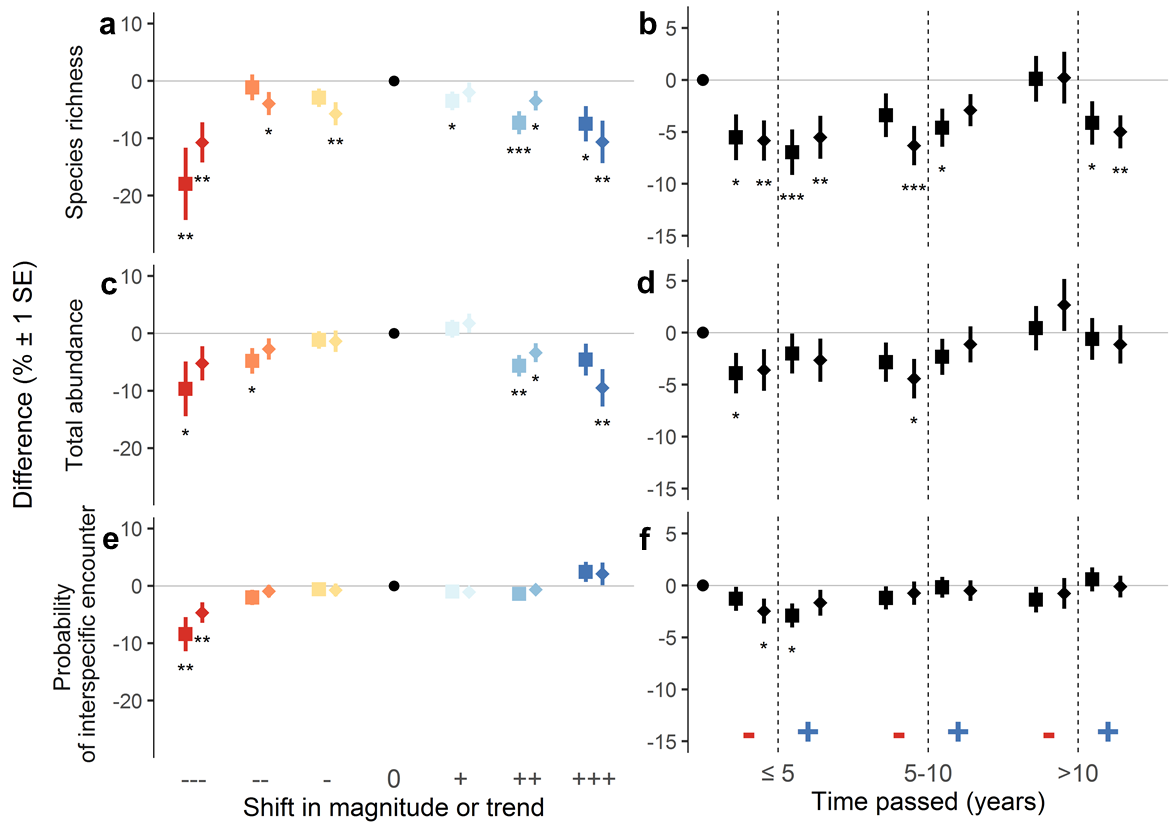
\includegraphics[width=1\textwidth]{chapter3/F02}
\caption{Local biodiversity impacts varied with attributes of abrupt land change. Differences in three measures of local biodiversity, (\textbf{a},\textbf{b}) species richness, (\textbf{c},\textbf{d}) total abundance, and (\textbf{e},\textbf{f}) the probability of interspecific encounter (PIE) at sites with an abrupt land change (squares, diamonds) relative to unchanged sites (0, black points). (\textbf{a},\textbf{c},\textbf{e}) Estimates are given separately for shifts in magnitude (squares; > 50\%, > 25\% to $\leq$ 50\%, and $\leq$ 25\% EVI loss [$---$ to $-$, coloured red to orange] or gain [$+++$ to $+$, blue to light blue], Appendix Figure \ref{SI03_02}\textbf{a}) or in EVI trend (diamonds; from $---$ to $+++$ for negative to positive trend differences, Appendix Figure \ref{SI03_02}\textbf{b}). (\textbf{b},\textbf{d},\textbf{f}) Impacts on biodiversity measures of time passed between an abrupt land change (gain/increase [$+$] or loss/decrease [$-$] in EVI shift in magnitude [squares] or trend [diamonds]) and sampling of biodiversity. Separate models were fitted for shifts in magnitude and in trend relative to unchanged sites (points). Error bars show fitted standard errors and asterisks statistical significance (* p < 0.05, ** p < 0.01, *** < 0.001) from the hierarchical models. For number of sites and studies for each bin and biodiversity measure see Appendix Figure \ref{SI03_04} and Table \ref{SIT03_01}}
\label{F03_02}
\end{figure}
% -------------------------------------------- %


\section{Results}
Local biodiversity measures are lower at sites with an abrupt land change in the past. Sites at which an abrupt land change was observed contained on average -4.2\% fewer species (SE: 1.3\%, $\chi^2$ = 10.27, df = 3, p < 0.01), -2\% fewer individuals (SE: 1.3\%; $\chi^2$ = 72.9, df = 3, p < 0.001), and species assemblages were -1\% less even (SE: 0.6\%; $\chi^2$ = 42.79, df = 3, p < 0.001) compared to unchanged sites (Figure 2). Sites with larger abrupt shifts in magnitude and trend had fewer species and individuals than unchanged sites regardless of direction of abrupt land change (Figure \ref{F03_02}\textbf{a},\textbf{c}). Sites with > 50\% loss or gain in EVI had on average -18\% (SE: 6.4\%) or -9\% (SE: 3.2\%) fewer species, and -10\% (SE: 5\%) or -5\% (SE: 3\%) fewer individuals than unchanged sites (Figure \ref{F03_02}\textbf{a},\textbf{c}). Compared to unchanged sites, species assemblages were less even at sites with larger abrupt losses in EVI, but not at sites with larger gains in EVI (Figure \ref{F03_02}\textbf{e}). We found similar impacts of shifts in magnitude and trend on species richness ($\Delta$AIC = 3.22, Pearson’s r between impacts = 0.71), abundance ($\Delta$AIC = 2.64, r = 0.61), and evenness ($\Delta$AIC = 5.66, r = 0.98).

Biodiversity can recover after an abrupt land change depending on time passed. We hypothesize that with more time passed local biodiversity recovers to levels comparable to unchanged sites. In line with our expectation we found that sites with an abrupt land change up to five years before biodiversity sampling had on average -6.6\% fewer species (SE: 1.8\%), -3\% fewer individuals (SE: 1.8\%) and were -2\% less even (SE: 0.1\%) than unchanged sites (Figure \ref{F03_02}\textbf{b},\textbf{d},\textbf{f}). After more than 10 years had passed, biodiversity measures were comparable to unchanged sites (Figure \ref{F03_02}\textbf{b},\textbf{d},\textbf{f}), except for local species richness at sites with positive shifts in magnitude or trend (-4\%; Figure \ref{F03_02}\textbf{b}). Overall, we found similar impacts of shifts in magnitude and trend and varying time passed for species richness ($\Delta$AIC = 2.85, Pearson’s r between impacts r = 0.66), abundance ($\Delta$AIC = 2.46, r = 0.42), and evenness ($\Delta$AIC = 3.03, r = 0.65).

% ---------------- Figure 3 --------------------- %
\begin{figure}[ht]
\centering
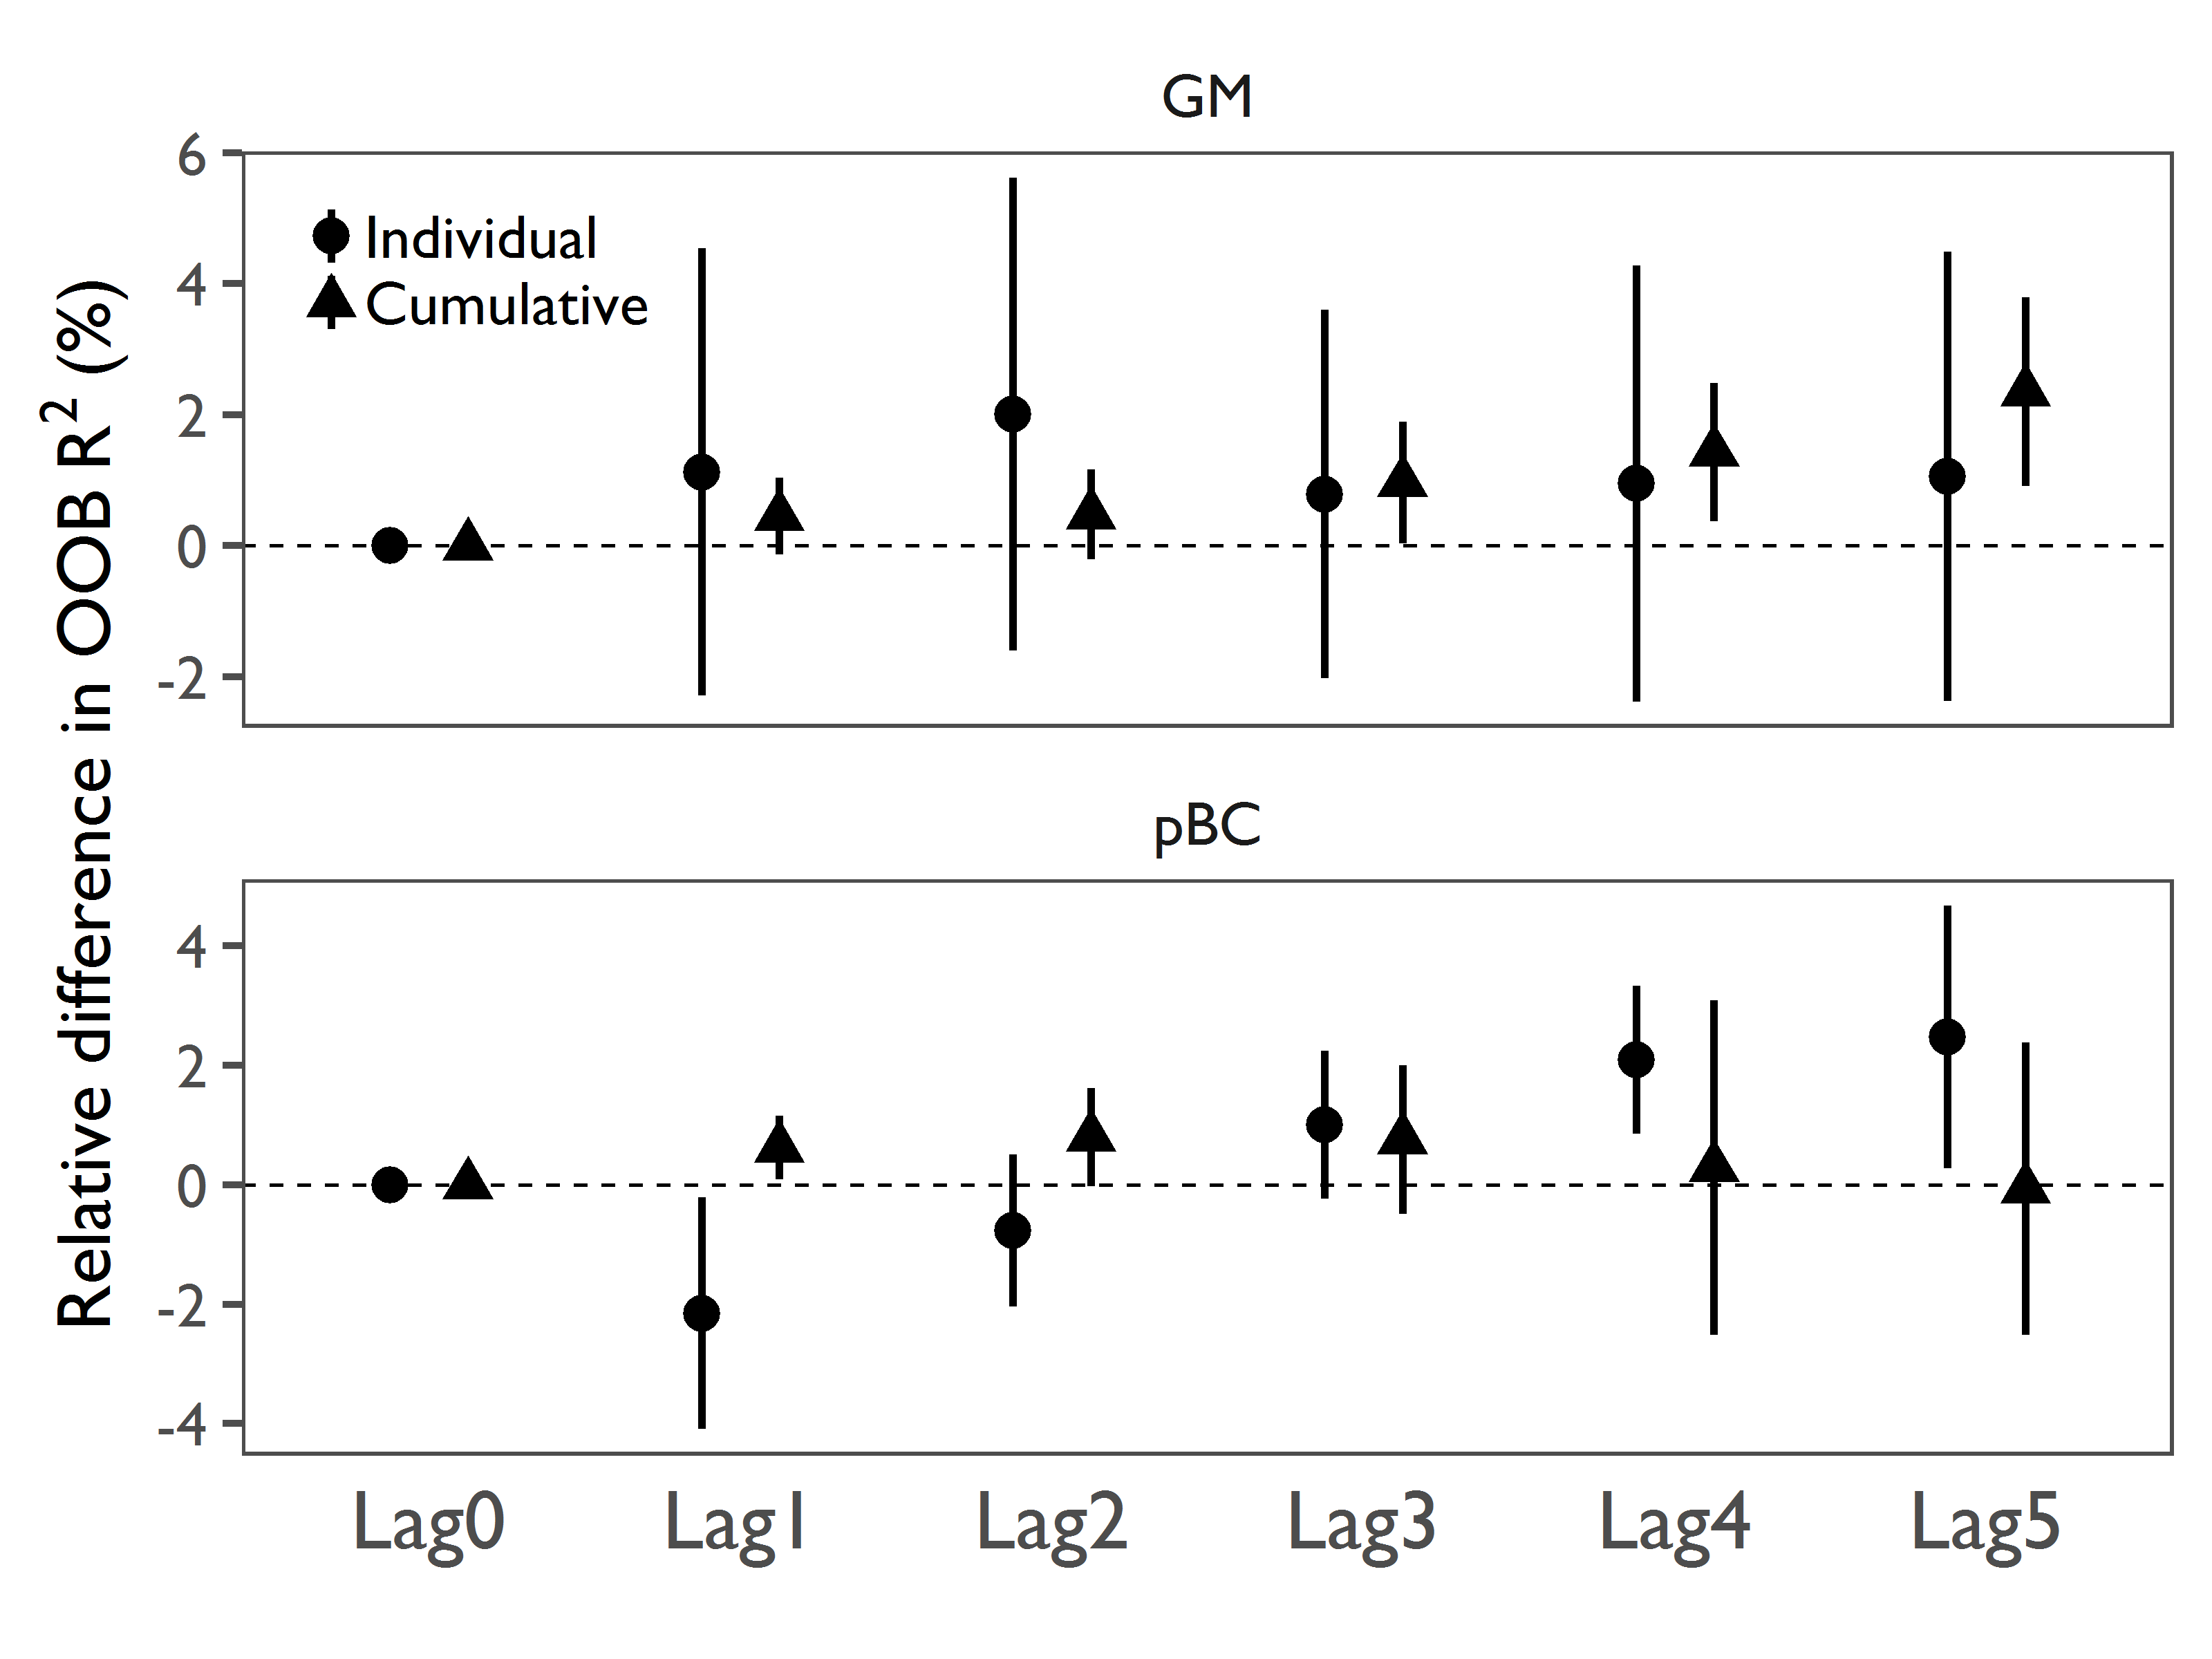
\includegraphics[width=1\textwidth]{chapter3/F03}
\caption{Reduced compositional similarity between sites without and with an abrupt land change. Mean similarity in species assemblage composition (S\o rensen similarity index) calculated between pairs of sites within the same study and land-use category without ($0$) and with an abrupt land change of (\textbf{a}, \textbf{c}) varying shifts in magnitude, or (\textbf{b}, \textbf{d}) loss or gain in EVI ($-$ and $+$) and time passed between abrupt land change and biodiversity sampling (axis labels as in Figure \ref{F03_02}). Colours indicate whether similarity of species assemblages was on average greater (purple) or smaller (brown) relative to unchanged sites. Numbers (in \textbf{a},\textbf{b}) indicate the total number of studies for which pairwise comparisons between sites could be made. All estimates are transformed relative to the compositional similarity between pairs of sites without a land change ($0 - 0$). (\textbf{c},\textbf{d}) Dendrograms show hierarchical clustering of all pairwise similarities based on the average Manhattan distance between pairs of sites; sites with more similar assemblage composition are in branches of closer proximity. }
\label{F03_03}
\end{figure}
% -------------------------------------------- %

Abrupt land change affects the composition of species assemblages. Species assemblages at sites with larger abrupt shifts in magnitude were less similar in composition to unchanged sites (Figure \ref{F03_03}\textbf{a}, \textbf{c}). Especially sites with a shift in magnitude of > 50\% EVI loss or gain were on average less similar (-0.12 / -0.03, respectively) in assemblage composition to unchanged sites (Figure \ref{F03_03}\textbf{a}). Furthermore, the composition of species assemblages was most dissimilar to unchanged sites if an abrupt land change occurred less than five years ago (Figure \ref{F03_03}\textbf{b},\textbf{d}). After more than five years had passed between an abrupt land change and biodiversity sampling, species assemblages were on average more similar in composition (0.04 / 0.001 for loss and gain in EVI, respectively) to unchanged sites (Figure \ref{F03_03}\textbf{b}). The composition of species assemblages was on average more similar among sites of comparable shifts in magnitude or with time passed (diagonals in Figure \ref{F03_03}\textbf{a},\textbf{b}) relative to unchanged sites. The impacts of abrupt shifts in magnitude were broadly comparable to shifts in trends although negative shifts in trend impacted assemblage composition more (Appendix Figure \ref{SI03_05}).

% ---------------- Figure 4 --------------------- %
\begin{figure}[!htb]
\centering
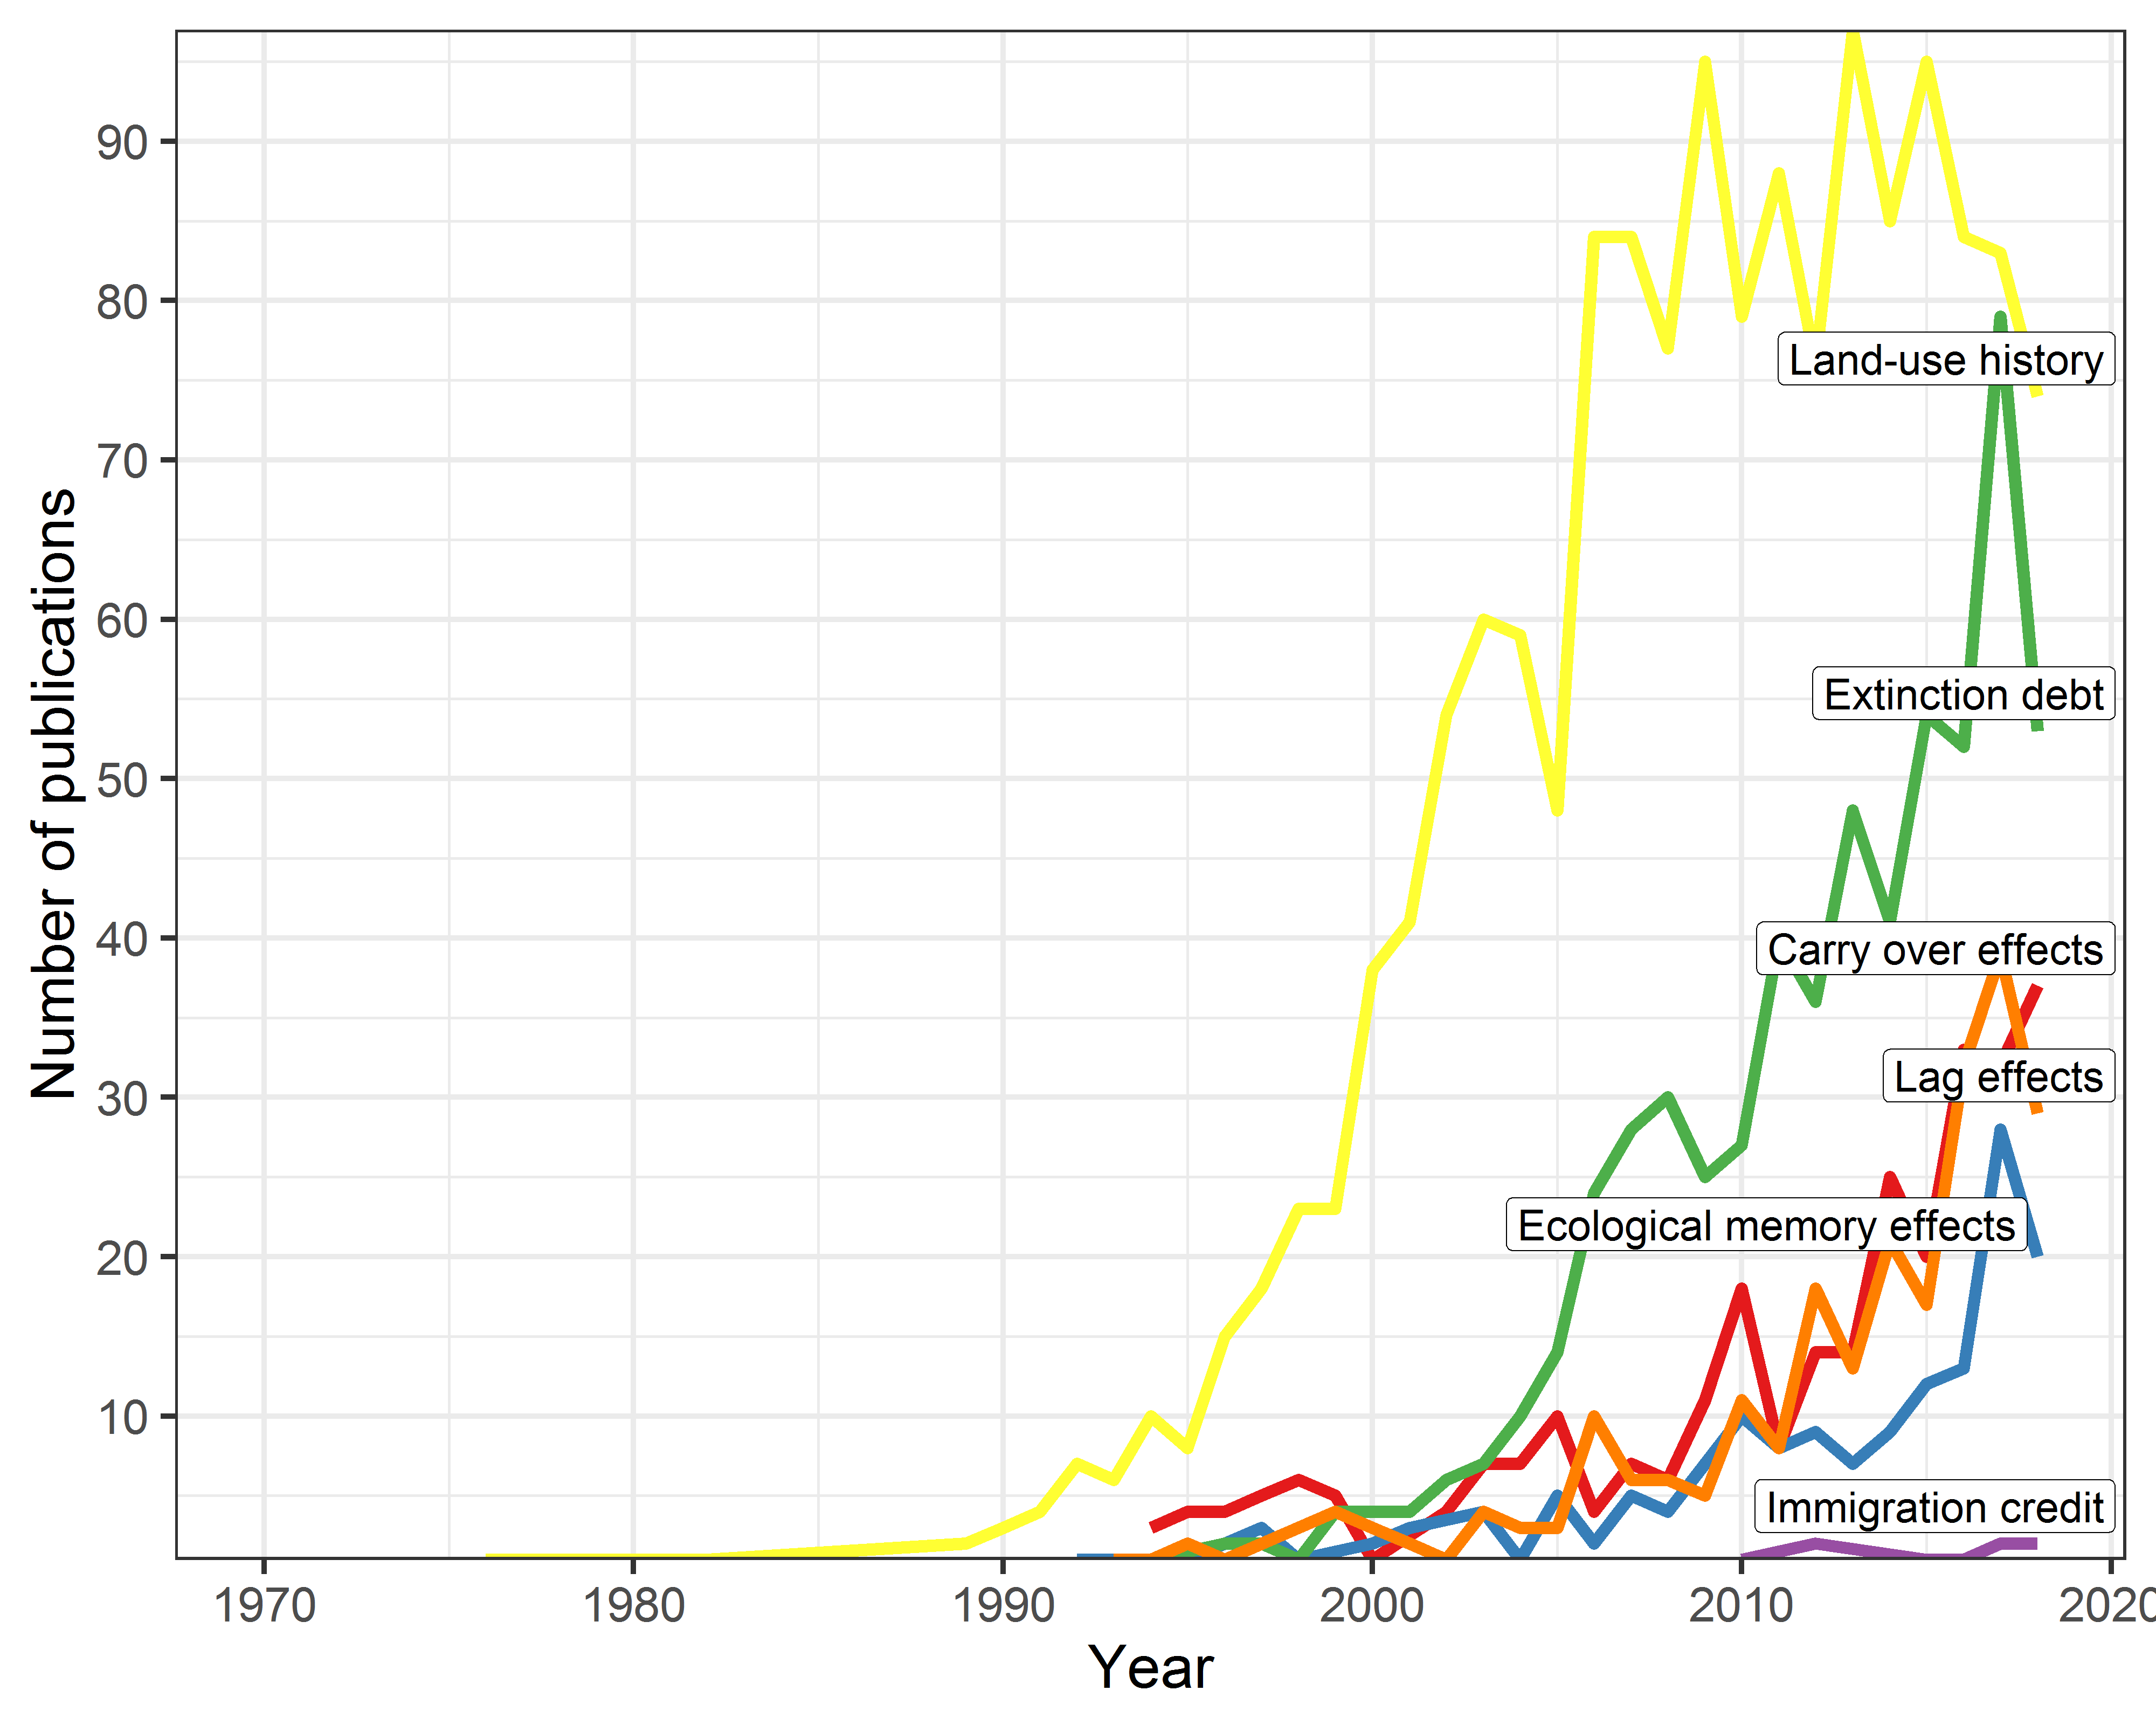
\includegraphics[width=1\textwidth]{chapter3/F04}
\caption{Abrupt land change affects taxonomic groups differently. Difference in (\textbf{a}) species richness, (\textbf{b}) total abundance, and (\textbf{c}) assemblage evenness for taxonomic groups (plants, fungi, ground dwelling invertebrates, flying invertebrates, amphibians, reptiles, birds, and mammals) between sites without and with an abrupt land change. Separate models were fitted for taxonomic groups comparing sites with shifts in magnitude (squares) and trend differences (diamonds) where colours indicate negative (red) and positive (blue) direction and sites without abrupt land change (black points, grey line). Error bars show standard errors and asterisks indicate statistical significance (* p < 0.05, ** p < 0.01, *** < 0.001). Numbers give the number of studies included per taxonomic group.}
\label{F03_04}
\end{figure}
% -------------------------------------------- %

Impacts of abrupt land changes in the past varies among taxonomic groups. Sites with a positive shift in magnitude had significantly fewer species of plant (-9.7\%), bird (-4.2\%), ground dwelling invertebrate (-6.4\%), and reptile (-10.4\%) compared to unchanged sites (Figure \ref{F03_04}\textbf{a}). Particularly sites with a negative shift in trend had significantly fewer species of plant (-8.2\%, Figure \ref{F03_04}\textbf{a}) and fungi (-29.6\%), and fewer individuals of fungi (-17.8\%, Figure \ref{F03_04}\textbf{b}) compared to unchanged sites. The number of individuals and assemblage evenness was overall lower at sites with an abrupt land change compared to unchanged sites, although amphibian and mammal abundance as well as evenness of flying insects was higher at sites with an abrupt land change (Figure \ref{F03_04}\textbf{b},\textbf{c}). For most taxonomic groups, except fungi and reptiles, there was little difference between the impacts of shifts in magnitude or trend on biodiversity measures (Figure \ref{F03_04}).

\section{Discussion}
We found species assemblages to be negatively impacted by past abrupt land change. Larger changes on land caused greater reductions in local biodiversity (Figure \ref{F03_02}\textbf{a}-\textbf{c}) regardless of whether shifts in magnitude or trend of photosynthetic activity (EVI) were positive or negative, suggesting general impacts of past abrupt land change on biodiversity \citep{Dornelas2010,Hautier2015} likely caused by biotic lag effects \citep{Hylander2013,Ogle2015,Jung2018}. Abrupt land changes with large (>50\%) losses or gains in EVI have caused immediate and time-delayed local extinctions \citep{Krauss2010,Halley2016,Wood2017}, and reduced the abundance and dominance of persisting species (Figure \ref{F03_02}\textbf{b}-\textbf{c}), which may ultimately affect ecosystem functioning \citep{Hautier2015,Isbell2015}. Previous studies predicted assemblage evenness to increase with change magnitude \citep{Svensson2012}, however our results demonstrate this to be only the case for positive changes in photosynthetic activity (\ie. a gain or positive trend shift in EVI). Abrupt land changes can alter the composition of species assemblages with early colonizing and non-native species often outperforming or replacing many persisting species \citep{Fraterrigo2006,Turner2010,Jauni2015}, which could explain the observed impacts on species assemblage evenness (Figure \ref{F03_02}\textbf{c}) and compositional similarity (Figure \ref{F03_03}).

The recovery from abrupt land change is of important concern for biodiversity conservation \citep{Chazdon2003}. We found biodiversity measures to be lower (Figure \ref{F03_02}\textbf{b},\textbf{d},\textbf{f}) and the composition of species assemblages altered more compared to unchanged sites (Figure \ref{F03_03}\textbf{b},\textbf{d}) if an abrupt land change occurred relatively recently (< 5 years). An explanation could be that some, disturbance sensitive, species are immediately lost from local assemblages because of an abrupt land change \citep{Devictor2008,Supp2014}. However local biodiversity can recover from an abrupt land change with biodiversity measures being comparable to unchanged sites after >10 years \citep{Martin2013,Moreno-Mateos2017}, although local species richness did not recover at sites where EVI had increased (Figure \ref{F03_02}\textbf{b}). Land changes causing an abrupt positive shift could be related to increase or sudden cessation of anthropogenic use intensity \citep{Eastman2013,Muller2014}, which may have caused further local species loss \citep{Tilman1994,Balmford1996,Hylander2013}. Nevertheless, the time passed since an abrupt land change occurred can be a poor predictor of biodiversity recovery as land trajectories are often highly unpredictable \citep{Norden2015} or include multiple land changes \citep{Watson2014}. We suggest future analyses to consider how additional attributes, such as trajectories or frequency of land change \citep{Watson2014}, influence local biodiversity recovery. 

A number of other factors mediate the response of local biodiversity to land change \citep{Arroyo-Rodriguez2015}.  Previous studies demonstrated local biodiversity to recover quicker from an abrupt land change with a greater availability of undisturbed land in the wider landscape \citep{Turner1989,Chase2003,Shackelford2017}. In addition, site-specific factors and a long history of human modification can mediate the impact of abrupt land change on local biodiversity \citep{Ellis2015a,Jung2016}, especially since the majority of sites in the PREDICTS database are in regions that have long been subjected to human influence \citep{Newbold2016,Hudson2016}. It is likely that some species – those particularly sensitive to land changes – have been lost from local assemblages long before the availability of Landsat data (< 1982) and we expect the found impacts of abrupt land change on biodiversity to be conservative \citep{Mihoub2017}. Land changes can also be characterized by attributes not considered in this study, such as frequency and trajectory \citep{Watson2014}, which have been shown to influence local biodiversity \citep{Tiemann2015,Wood2017} and for many types of land change events - such as harvests, grazing or fallow period cycles \citep{Kleyer2007,Ray2013} - are often similar in shifts of magnitude and trend. Future studies should evaluate the influence of differing land trajectories and frequencies of land change on local biodiversity.

What drives abrupt land change events? Abrupt land change, identified by shifts in magnitude and/or trend of photosynthetic activity, can be caused by anthropogenic deforestation \citep{DeVries2015b}, land intensification \citep{Fensholt2012,Muller2014}, or degradation \citep{Tian2015,Aguiar2017}. In this study we did not separate between natural and anthropogenic drivers of abrupt land change and changes in photosynthetic activity can also be caused by rainfall-driven anomalies \citep{Papagiannopoulou2017} or changing nitrogen deposition and CO2 fertilization \citep{Zhu2016}. Most PREDICTS sites are modified by humans \citep{Newbold2016,Hudson2016} and it is therefore likely that most detected land changes were caused by humans. Future studies should attempt to distinguish and disentangle the impacts of natural and anthropogenic abrupt land changes \citep{Curtis2018}. 

Detecting and quantifying abrupt land changes is challenging. Here we focussed on detecting abrupt land change as shifts in magnitude or trend \citep{Verbesselt2010a}, but not all land change is abrupt \citep{Vogelmann2012a} or - such as understory thinning and selective logging - can be detected in time series of remotely-sensed photosynthetic activity \citep{Asner2005,Peres2006}. Similar to previous studies we assessed only the impact of the single largest shift in magnitude or trend \citep{DeJong2013,Song2018}, while different sequences of land change may also affect local biodiversity \citep{Watson2014}. Future studies quantifying abrupt land change globally could benefit from better access to, or fusion of, available satellite data to reach higher temporal and spectral resolution \citep{Reiche2015,Wulder2015}.

In conclusion, we demonstrate that compared to unchanged sites local biodiversity is considerably reduced because of abrupt land changes in the past, potentially affecting the stability and functioning of ecosystems \citep{Hautier2015}. Ignoring delayed biodiversity responses to abrupt land changes means that contemporary biodiversity changes, loss and recovery, are underestimated \citep{Kuussaari2009,Essl2015}. Conservation practitioners need to consider the impacts of biotic lag effects to ensure global and regional assessments (e.g. those by the Intergovernmental Science-Policy Platform on Biodiversity and Ecosystem Services [IPBES]) fully capture biodiversity change \citep{Essl2015}. Remote sensing can assist in quantifying attributes of abrupt land change over large spatial and temporal scales. Our analytical framework can be expanded to assess spatial prioritization of habitat restoration plans or to support scenario-based modelling \citep{Ewers2009} to predict the impacts of abrupt land change on local biodiversity.

\section{Data and code availability}
The PREDICTS biodiversity data are publicly available in the Natural History Museum Data Portal (\doi{10.5519/0066354}, \cite{Hudson2016}). All remote sensing data are accessible via Google Earth Engine (\href{earthengine.google.com/}{earthengine.google.com/}) \citep{Gorelick2017} and pre-processed time series will be deposited on GitHub (\href{https://github.com/Martin-Jung/PastDisturbance}{https://github.com/Martin-Jung/PastDisturbance}) on publication.Data and code to reproduce the results will be made available in a GitHub repository (\href{https://github.com/Martin-Jung/PastDisturbance}{https://github.com/Martin-Jung/PastDisturbance}) on publication.

\clearpage
%\bibliography{content/04Chapter}

%\appendix
%\begingroup
%  % SI - Figure 1 Missing data
\begin{figure}[h]
\centering
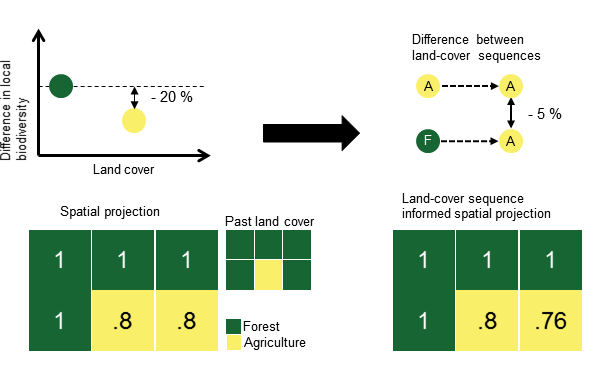
\includegraphics[width=1\textwidth]{chapter3/SI01}
\caption{ Average temporal distribution of Landsat data and an example times series of Landsat data. (\textbf{a}) Distribution of available Enhanced Vegetation Index (EVI) data in years covered by the Landsat missions. Points show the average monthly EVI data availability per year (0 to 12 months of data) across time series and PREDICTS sites grouped by 15\textdegree latitude bins. The size of points indicates the mean data availability (0 to 100\% with 100\% having 12 months of available data in a given year), while the colour shows the number of PREDICTS sites contributing to the mean (as PREDICTS sites were sampled in varying years). (\textbf{b}) Example time series for one PREDICTS site with a high proportion of missing data before 1999. In all analyses such time series were truncated to the period from 1999 onwards (indicated by the dashed line).}
\label{SI03_01}
\end{figure}

% SI - Figure 2 Binning
\begin{figure}[h]
\centering
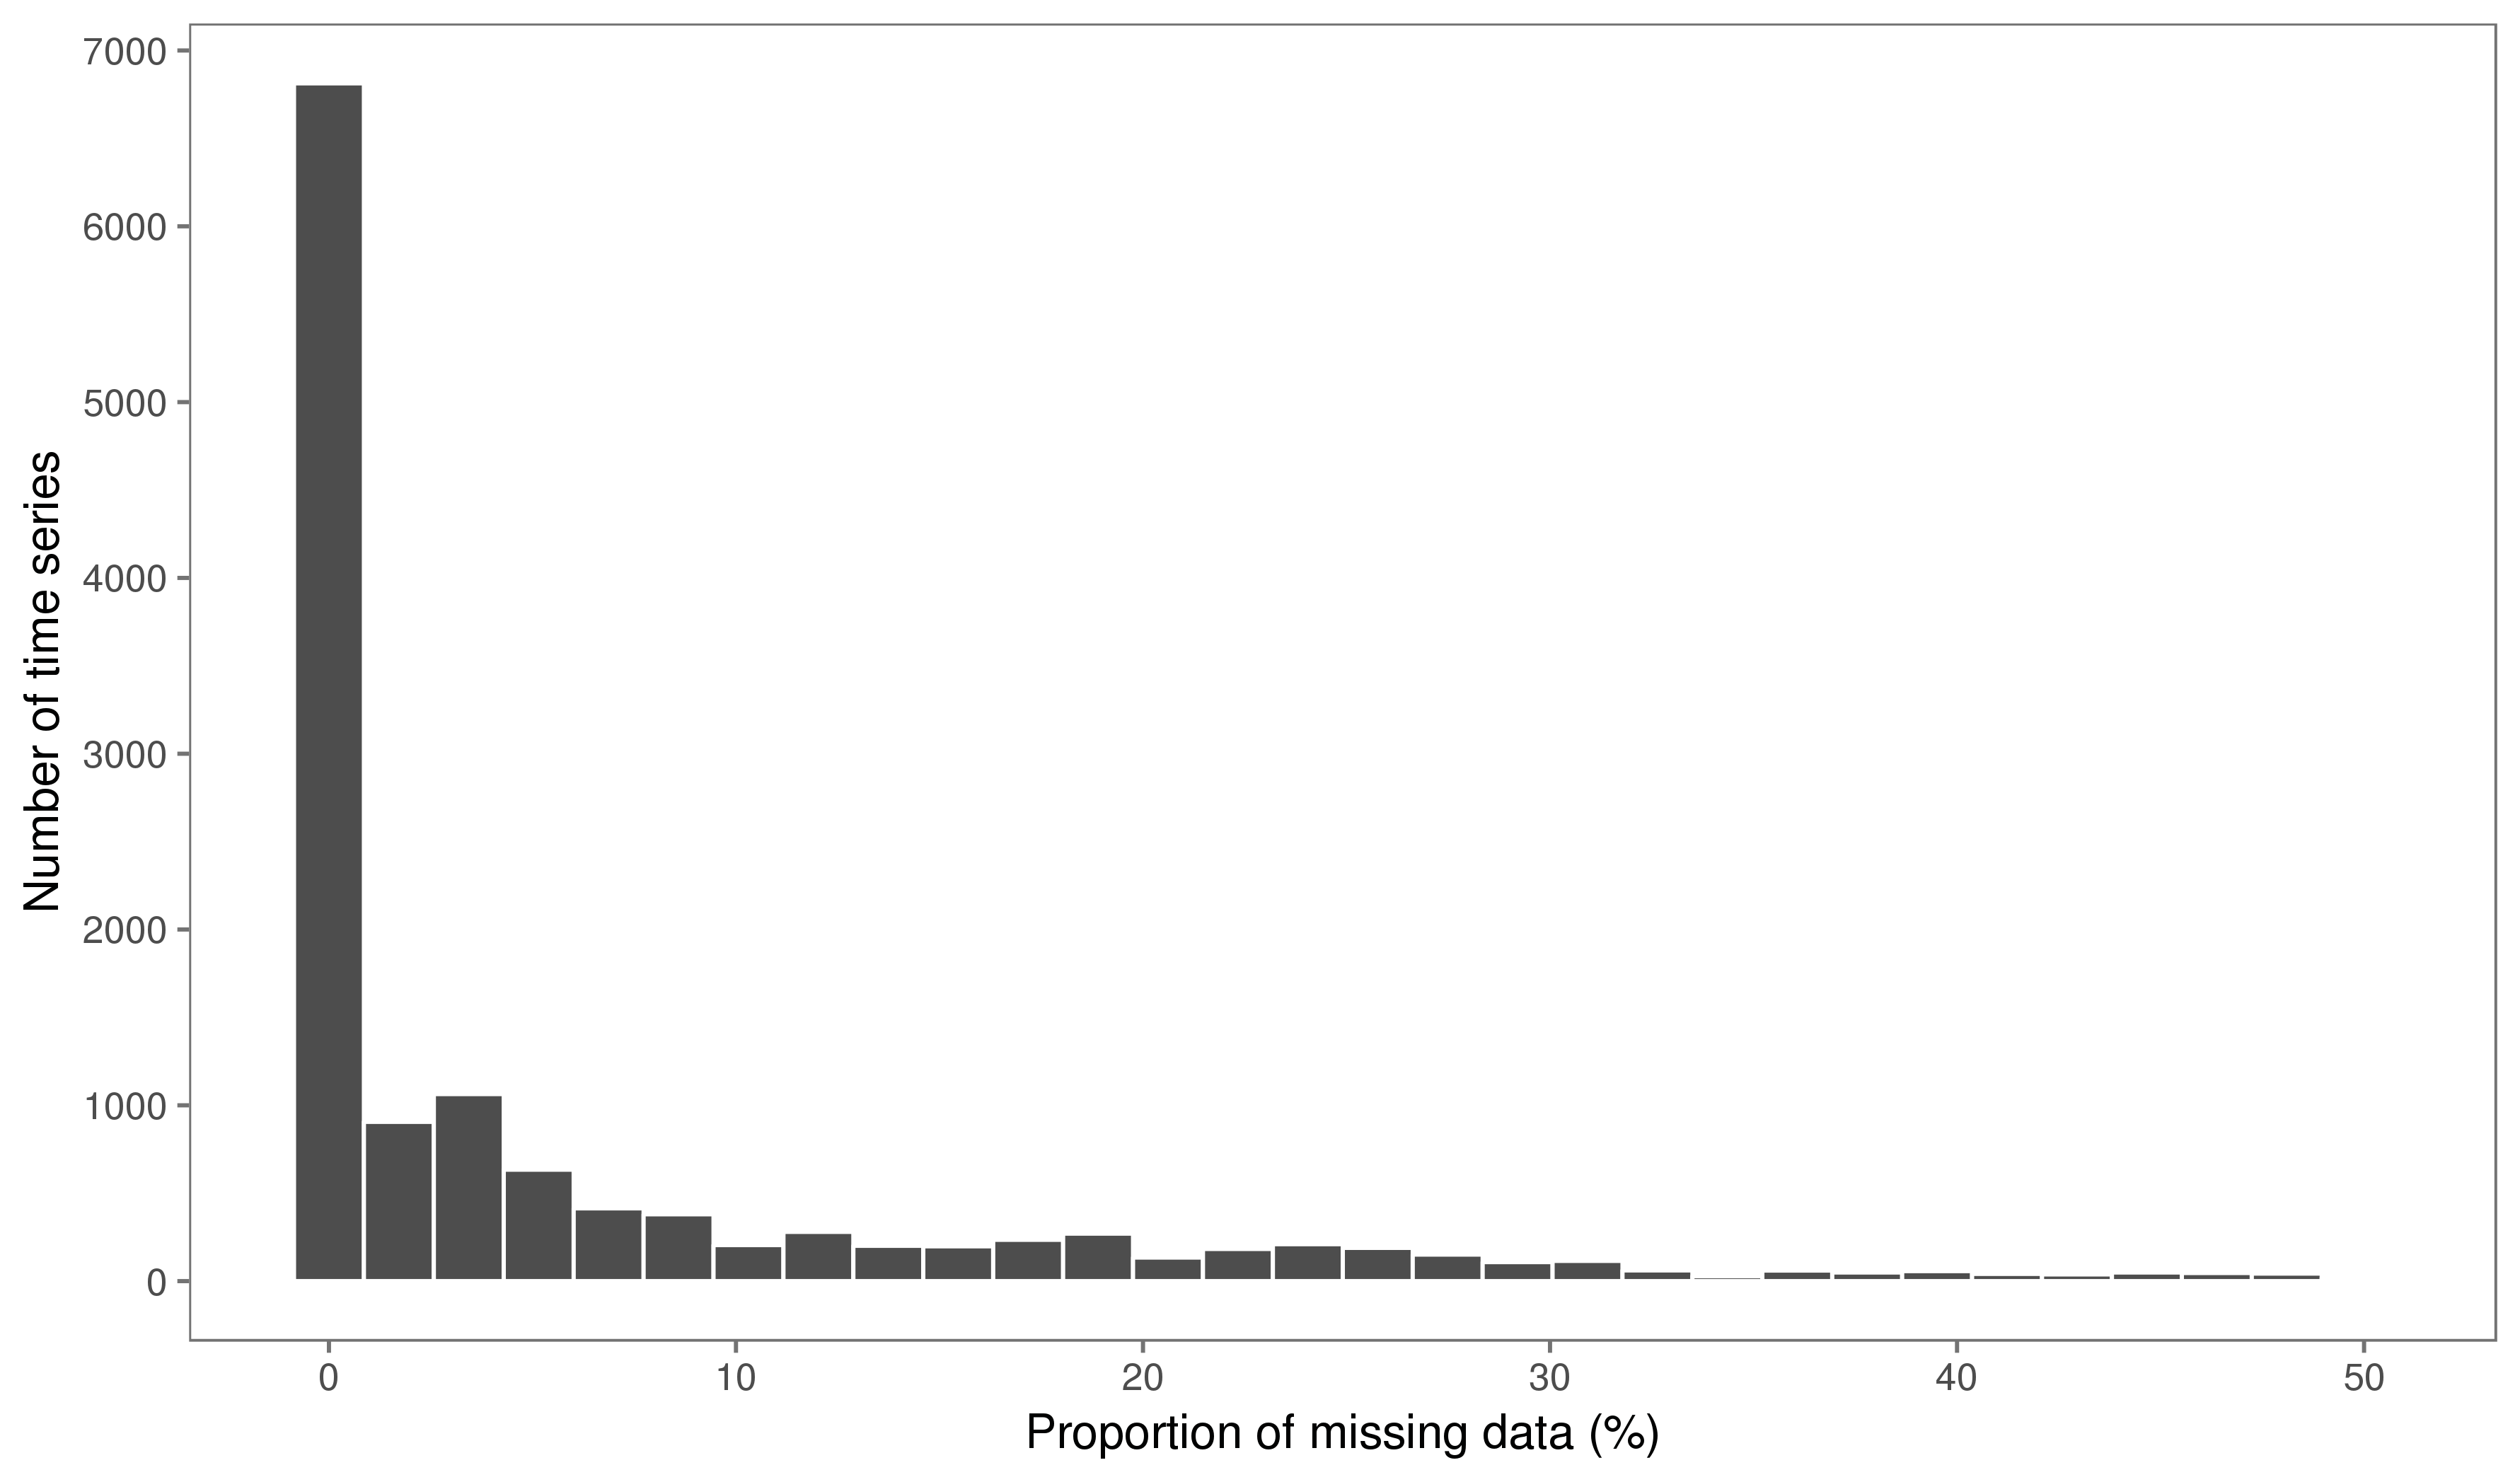
\includegraphics[width=1\textwidth]{chapter3/SI02}
\caption{ Number of sites with abrupt land change per attribute. Number of sites (black line) per attribute of abrupt land change with (\textbf{a}) the relative shift in magnitude, (\textbf{b}) the shift in trend as difference in annual EVI trend, and (\textbf{c}) the time passed between abrupt land change and biodiversity sampling. Background colours in (\textbf{a}) and (\textbf{b}) indicate the binning into six groups for shifts in magnitude (> 50\%, > 25\% to $\leq$ 50\%, and $\leq$ 25\% EVI loss [$---$ to $-$] or gain [$+++$ to $+$]), and in trend (0.01, 0.05, and > 0.05 annual negative [$---$ to $-$] to positive [$+++$ to $+$] EVI trend differences). Gray lines in (\textbf{c}) delineate bins of time passed ($\leq$ 5 years, > 5 and $\leq$ 10 years, and >10 years). Colours as in Figure \ref{F03_02}.}
\label{SI03_02}
\end{figure}

% SI Table 1------ %
% From here https://www.tablesgenerator.com/
\begin{table}[]
\centering
\caption{Number of PREDICTS sites and studies with an abrupt land change. Shown as either a change in magnitude (columns) and/or change in trend (trend). Symbols as in Figure \ref{F03_02}. }
\label{SIT03_01}
\begin{tabular}{@{}lllllllllll@{}}
                                          &                                           & \multicolumn{7}{c}{\textbf{Shift in magnitude}}                                                                                                                                                                    &                               &                             \\
                                          &                                           & \textbf{- - -}             & \textbf{- -}                & \textbf{-}                   & \textbf{0}                    & \textbf{+}                   & \textbf{+ +}                & \textbf{+ + +}              & \textbf{Total sites}          & \textbf{Studies}            \\ \cmidrule(l){3-11} 
                                          & \multicolumn{1}{l|}{- - -}                & 2                          & 8                           & 192                          & NA                            & 73                           & 26                          & 22                          & \cellcolor[HTML]{EFEFEF}323   & \cellcolor[HTML]{C0C0C0}57  \\
                                          & \multicolumn{1}{l|}{- -}                  & 7                          & 281                         & 642                          & NA                            & 497                          & 158                         & 53                          & \cellcolor[HTML]{EFEFEF}1638  & \cellcolor[HTML]{C0C0C0}175 \\
                                          & \multicolumn{1}{l|}{-}                    & 7                          & 88                          & 256                          & NA                            & 231                          & 154                         & 53                          & \cellcolor[HTML]{EFEFEF}789   & \cellcolor[HTML]{C0C0C0}184 \\
                                          & \multicolumn{1}{l|}{0}                    & NA                         & NA                          & NA                           & 10102                         & NA                           & NA                          & NA                          & \cellcolor[HTML]{EFEFEF}10102 & \cellcolor[HTML]{C0C0C0}358 \\
                                          & \multicolumn{1}{l|}{+}                    & 9                          & 102                         & 399                          & NA                            & 410                          & 205                         & 49                          & \cellcolor[HTML]{EFEFEF}1174  & \cellcolor[HTML]{C0C0C0}237 \\
                                          & \multicolumn{1}{l|}{\textbf{+ +}}         & 47                         & 172                         & 342                          & NA                            & 465                          & 254                         & 86                          & \cellcolor[HTML]{EFEFEF}1366  & \cellcolor[HTML]{C0C0C0}224 \\
\multirow{-7}{*}{\textbf{\rotatebox{90}{Shift in trend}}} & \multicolumn{1}{l|}{\textbf{+ + +}}       & 12                         & 137                         & 47                           & NA                            & 34                           & 12                          & 31                          & \cellcolor[HTML]{EFEFEF}273   & \cellcolor[HTML]{C0C0C0}56  \\
                                          & \multicolumn{1}{l|}{\textbf{Total sites}} & \cellcolor[HTML]{EFEFEF}84 & \cellcolor[HTML]{EFEFEF}788 & \cellcolor[HTML]{EFEFEF}1878 & \cellcolor[HTML]{EFEFEF}10102 & \cellcolor[HTML]{EFEFEF}1710 & \cellcolor[HTML]{EFEFEF}809 & \cellcolor[HTML]{EFEFEF}294 &                               &                             \\
                                          & \multicolumn{1}{c|}{\textbf{Studies}}     & \cellcolor[HTML]{C0C0C0}34 & \cellcolor[HTML]{C0C0C0}135 & \cellcolor[HTML]{C0C0C0}246  & \cellcolor[HTML]{C0C0C0}358   & \cellcolor[HTML]{C0C0C0}263  & \cellcolor[HTML]{C0C0C0}171 & \cellcolor[HTML]{C0C0C0}83  &                               &                            
\end{tabular}
\end{table}
% ------ %

% SI - Figure 3 Cross-correlations
\begin{figure}[h]
\centering
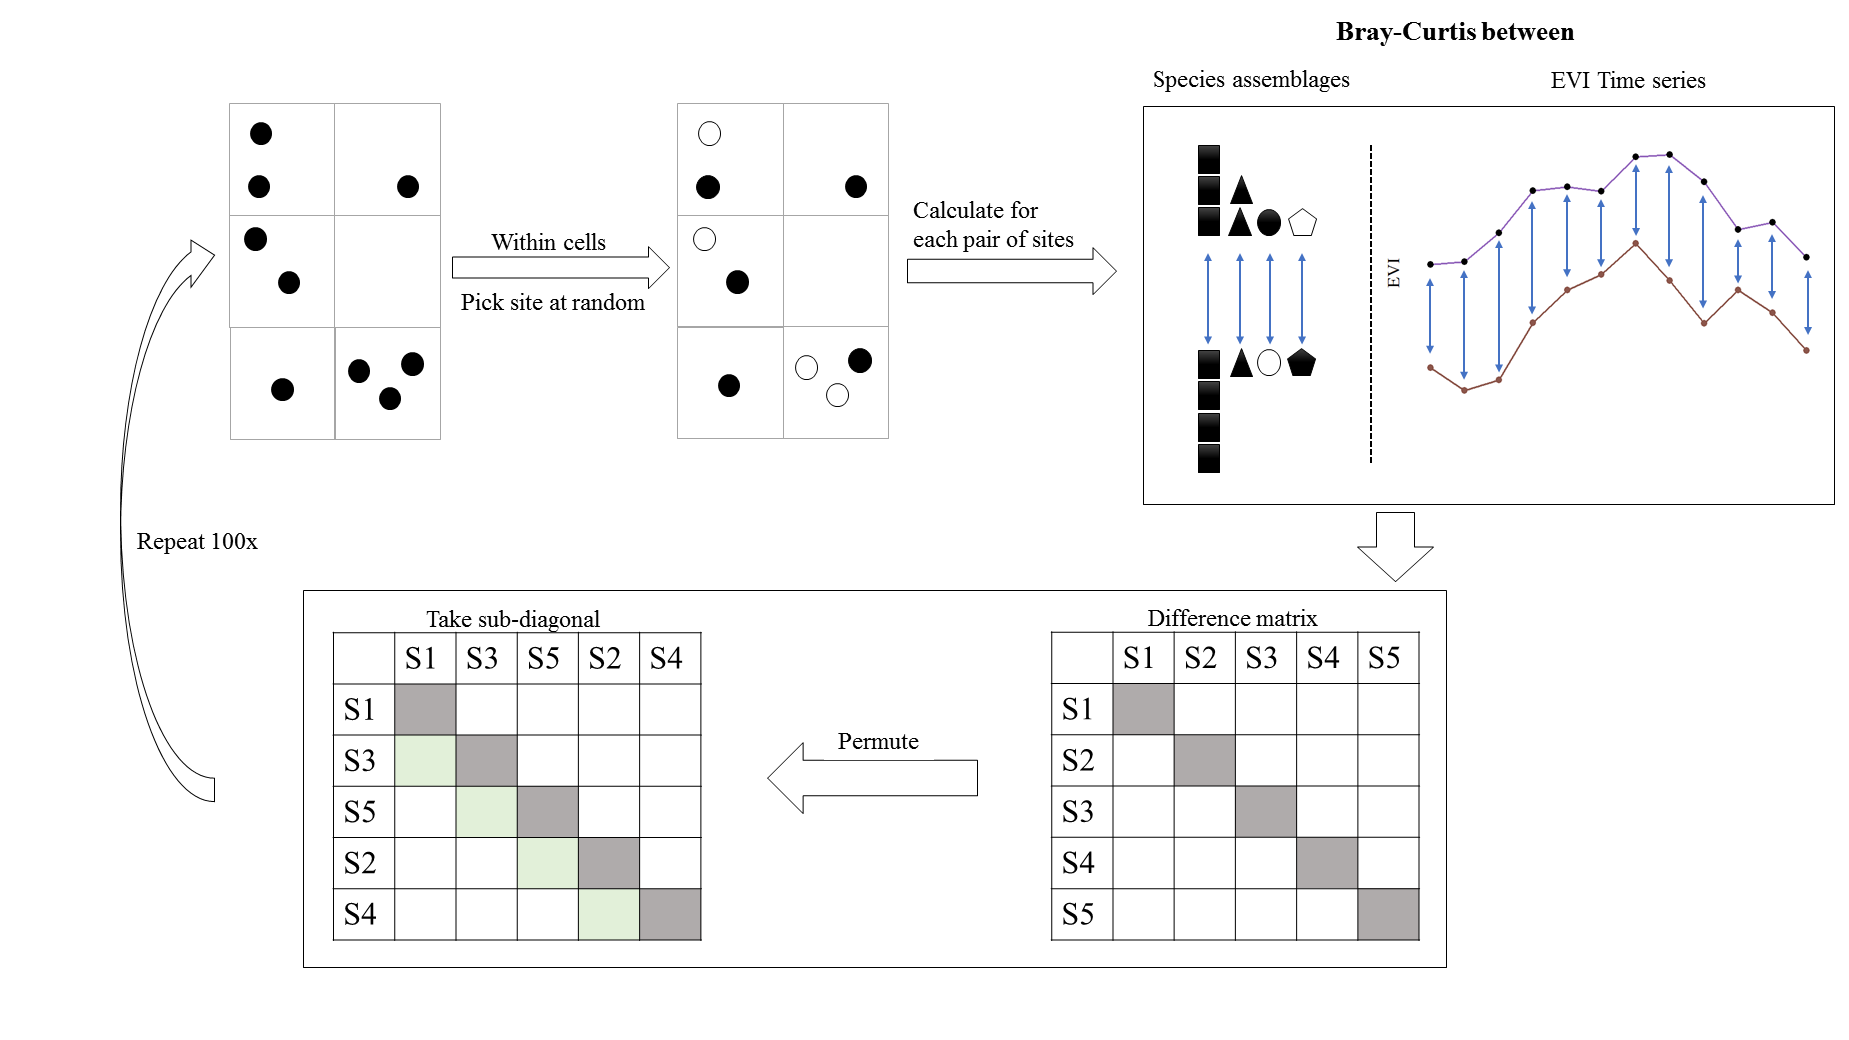
\includegraphics[width=1\textwidth]{chapter3/SI03}
\caption{ Correlations between attributes of abrupt land change. Showing shifts in magnitude, trend and time passed (see Methods). The lower facets show a point density plot, the upper facets the Pearson correlation coefficient between pairs of attributes and the diagonal a density plot.}
\label{SI03_03}
\end{figure}

%\endgroup
